\section{Motors}
An electric motor converts electrical power into mechanical rotation, that can turn the Wheels of HADES.
In this section will propose two different possible types of motors HADES could end up using.

\subsection{AC motor}
AC motors consist of two main part. A stator and a rotor. The stator is a stationary part and the rotor is a rotating part. The rotor is located inside of the stator and due to magnetic fields inside of the stator, the rotor will rotate\cite{motor21}.\\ 
AC motor use a alternating current see figure \ref{fig:ACmotor}. Due to the slip-rings, the AC motor provides energy to the robot\cite{motor21}.

\begin{figure}[h]
    \centering
    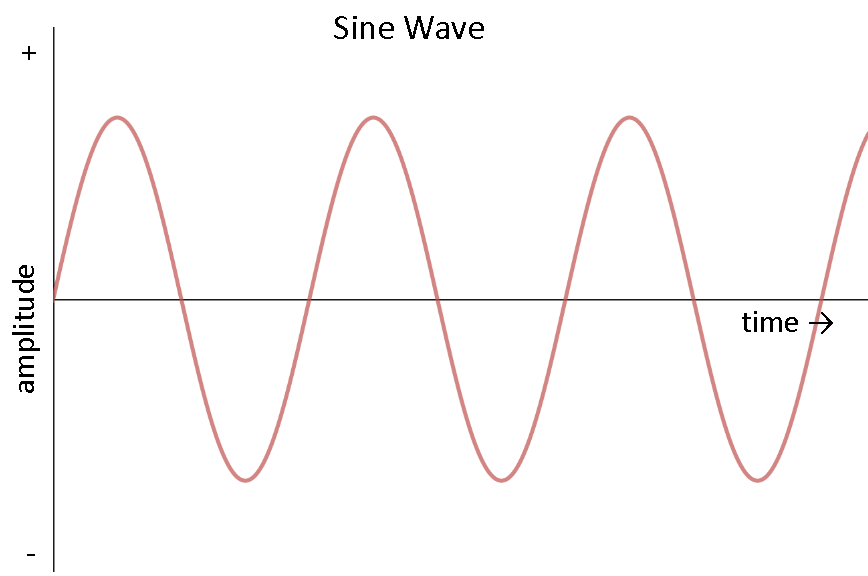
\includegraphics[width=.6\linewidth]{figures/wave.png}
    \caption{Alternative current\cite{ACmotor3}}
    \label{fig:ACmotor}
\end{figure}

\subsection{Brushless DC motor}
The working process of a brushless DC motor is similar to an AC motor. The main difference between a brushless DC motor and an AC motor is how they produce energy. Furthermore, brushless DC motors use commutator instead of slip rings to create a current energy.\\ 
The brushless DC motor have around 85\%-90\% efficiency.The advantage of brushless DC motor is less noisy\ref{fig:DCmotor}\cite{DCbrusshles}.

\begin{figure}[h]
    \centering    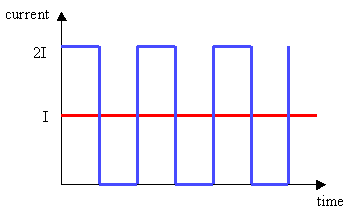
\includegraphics[width=.6\linewidth]{figures/dcMotor.png}
    \caption{Brushless DC curve angular\cite{Graphdd}}
    \label{fig:DCmotor}
\end{figure}

 %\newpage

\subsection{Conclusion} 
Brushless DC motors is more advance and controlling system are more simple than AC motor. In addition to this, HADES using brushless DC motor will be controlled easier.
